\documentclass{beamer}
\usepackage{beamerthemeshadow}
\usepackage[czech]{babel}
\usepackage[IL2]{fontenc}
\usepackage[utf8]{inputenc}
\usepackage{times}
\usepackage{hyperref}
\hypersetup{hidelinks}

\addtobeamertemplate{navigation symbols}{}{%
    \usebeamerfont{footline}%
    \usebeamercolor[fg]{footline}%
    \hspace{1em}%
    \insertframenumber/\inserttotalframenumber
}


\begin{document}

\title{Život a dílo Ayn Randové}  
\author{Matěj Hrabal}
\date{21.\,4.\,2017} 

\frame{
\titlepage
} 

\frame
{
\frametitle{Obsah}
\tableofcontents
} 

\section{Život} 
\frame{
\frametitle{Základní informace}
\begin{columns}
\begin{column}{.6\textwidth} 
\begin{itemize}
\item Pravým jménem Alisa Zinověvna Rosenbaum
\item Ruská spisovatelka a filosofka židovského původu
\item Autorka filosofie objektivismu
\end{itemize}
\end{column}
\begin{column}{.4\textwidth}
\begin{figure}
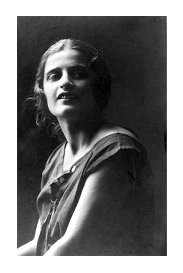
\includegraphics[scale=1.25]{Rand} 
\end{figure}
\end{column}
\end{columns}
}

\frame{ 
\frametitle{Důležité události} 
\begin{itemize}
\item Narozena 2.\,února\,1905, Rusko
\item První publikovaná monografie \uv{Pola Negri}, 1925
\item 19.\,února\,1926 emigruje do USA 
\item 1943 vydává knihu \uv{Fountainhead}, náznaky objektivismu
\item 1957 vydání díla \uv{Atlas Shrugged}, její magnum opus
\item Úmrtí 6.\,března\,1982, USA
\end{itemize} 
}

\section{Dílo} 
\subsection{The Fountainhead}
\frame{
\frametitle{The Fountainhead}
\begin{columns}
\begin{column}{.6\textwidth}
\begin{itemize}
\item Jedno z prvních úspěšných děl  
\item Psáno po dobu sedmi let
\item Filosofický román obsahující její politické názory
\item Poprvé zfilmován v roce 1949
\end{itemize} 
\end{column}
\begin{column}{.4\textwidth}
\begin{figure}
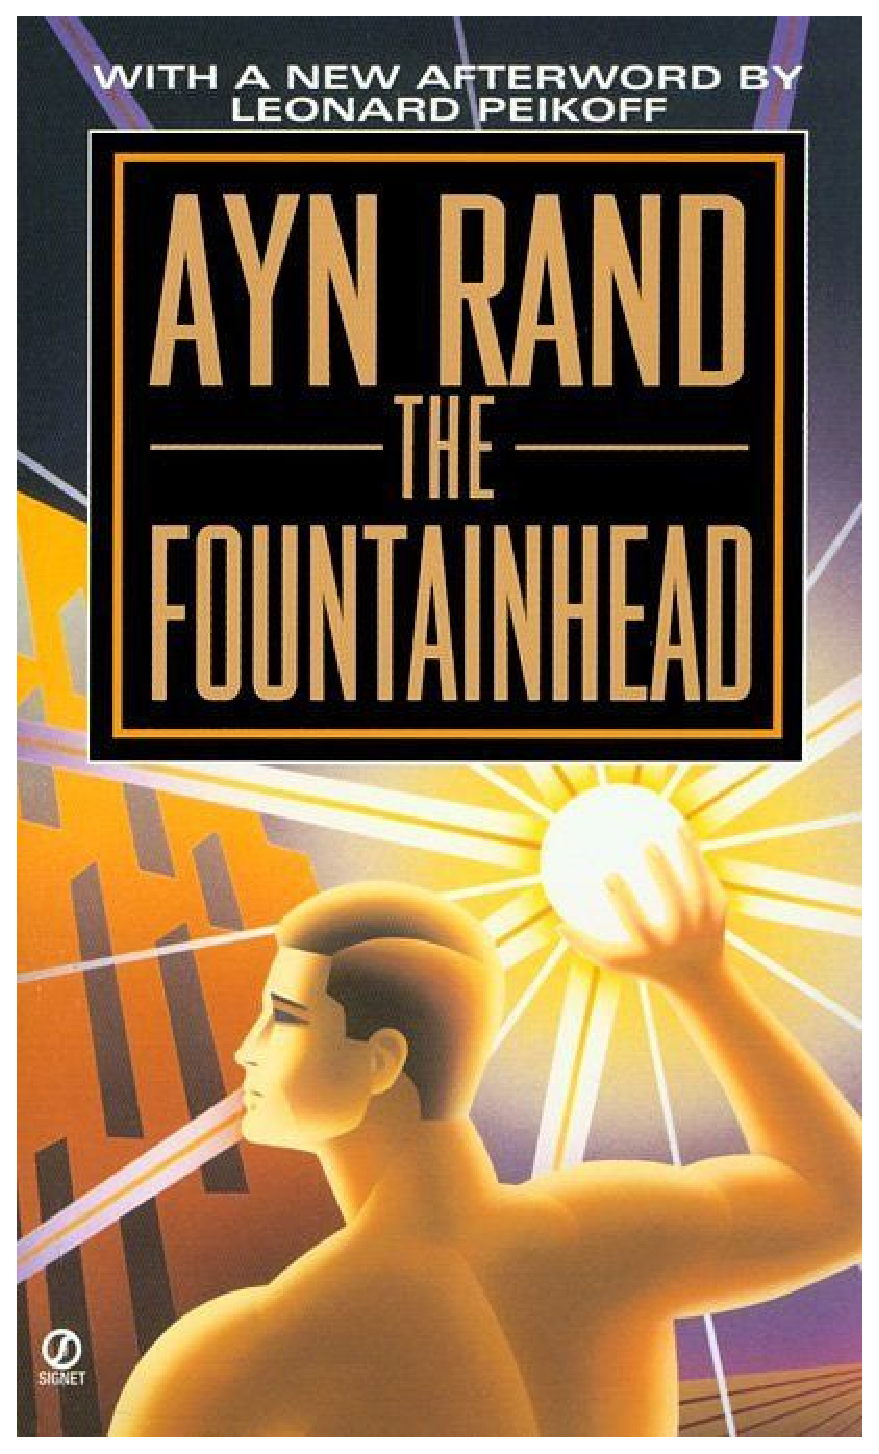
\includegraphics[scale=0.24]{Fountainhead} 
\end{figure}
\end{column}
\end{columns}
}

\subsection{Atlas Shrugged}
\frame{
\frametitle{Atlas Shrugged}
\begin{columns}
\begin{column}{.6\textwidth}
\begin{itemize}
\item Považován za \uv{magnum opus}
\item Mezinárodní bestseller 
\item Podle Randové pokračování knihy \uv{Fountainhead}
\item Poslední román kariéry
\item Po vydání Randová upadá do~depresí
\end{itemize}
\end{column}
\begin{column}{.4\textwidth}
\begin{figure}

\includegraphics[scale=1.41]{Atlas} 
\end{figure}
\end{column}
\end{columns}
}

\subsection{Další díla}
\frame{
\frametitle{Další díla}
\begin{itemize}
\item \uv{We the Living} (1936)  
\item \uv{Anthem} (1938)
\item Knihy zabývající se objektivismem
\end{itemize}
\begin{figure}
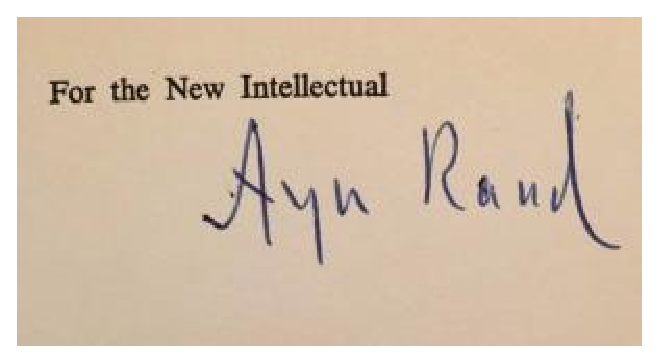
\includegraphics[scale=0.65]{Signature} 
\end{figure}
}

\section{Objektivismus} 
\frame{
\frametitle{Objektivismus}
\begin{itemize}
\item Systematická filosofie
\item Odsuzování etického altruismu
\item Částečně vychází z Aristotelova učení
\item Více popsán v knihách \uv{The Virtue of Selfishness} a~\uv{Capitalism: The Unknown Ideal}
\end{itemize}
}

\section{Použité zdroje}
\frame{
\frametitle{Zdroje}
\begin{itemize}
\item \url{https://en.wikipedia.org/wiki/Ayn_Rand} [online], vid.\,[21.\,4.\,2017]
\item \url{https://www.aynrand.org} [online], vid.\,[21.\,4.\,2017]
\item RAND, A.: The Fountainhead, ISBN~978-0141188621 
\item RAND, A.: Atlas Shrugged, ISBN~978-0451191144 
\end{itemize}
}

\frame{
\frametitle{Konec}
\center{\Huge{Děkuji za pozornost}}
}
\end{document}
